\documentclass[12pt,a4paper]{article}
\usepackage[a4paper, margin=0.8in, headheight=14pt]{geometry}
\usepackage{fontspec}
\usepackage{unicode-math}
\setmainfont{TeX Gyre Pagella}
\setmonofont[Scale=0.88]{TeX Gyre Cursor}
\setmathfont{Latin Modern Math}
\usepackage{xcolor}
\usepackage{colortbl}
\usepackage{titlesec}
\usepackage{enumitem}
\usepackage{tabularx}
\usepackage{booktabs}
\usepackage{array}
\usepackage{amsmath}
\usepackage{tikz}
\usetikzlibrary{shapes.geometric, arrows.meta, positioning, calc, fit, decorations.pathreplacing}
\usepackage{tcolorbox}
\tcbuselibrary{skins, breakable}
\usepackage{hyperref}
\usepackage{fancyhdr}
\usepackage{graphicx}
\usepackage{microtype}
\hyphenpenalty=10000
\exhyphenpenalty=10000
\sloppy
\usepackage{caption}
\usepackage{setspace}
\usepackage{multirow}
\usepackage{tocloft}
\newcommand{\Q}[1]{\textbf{#1}\par\noindent\ignorespaces}
\definecolor{myred}{RGB}{196,30,58}
\definecolor{mydark}{RGB}{30,30,50}
\definecolor{mygreen}{RGB}{14,120,80}
\definecolor{myteal}{RGB}{0,130,140}
\definecolor{myamber}{RGB}{180,100,0}
\definecolor{mypurple}{RGB}{100,30,160}
\definecolor{mygray}{RGB}{246,247,249}
\definecolor{mgframe}{RGB}{180,185,200}
\definecolor{watermark}{RGB}{145,150,170}
\definecolor{hdrred}{RGB}{250,232,235}
\definecolor{hdrgreen}{RGB}{220,244,233}
\definecolor{hdrteal}{RGB}{220,242,244}
\definecolor{hdramber}{RGB}{253,242,215}
\definecolor{hdrpurple}{RGB}{238,228,255}
\definecolor{hdrgray}{RGB}{238,240,245}
\definecolor{rowalt}{RGB}{250,251,253}
\titleformat{\section}{\large\bfseries\color{myred}}{\thesection.}{0.5em}{}[\vspace{1pt}{\color{myred}\rule{\linewidth}{0.8pt}}]
\titleformat{\subsection}{\normalsize\bfseries\color{myteal}}{\thesubsection}{0.5em}{}
\titlespacing*{\section}{0pt}{18pt}{7pt}
\titlespacing*{\subsection}{0pt}{11pt}{4pt}
\setlength{\parindent}{0pt}
\setlength{\parskip}{4pt}
\renewcommand{\cfttoctitlefont}{\large\bfseries\color{myred}}
\renewcommand{\cftaftertoctitle}{\par\noindent{\color{myred}\rule{\linewidth}{0.8pt}}}
\setlength{\cftbeforetoctitleskip}{0pt}
\setlength{\cftaftertoctitleskip}{6pt}
\renewcommand{\cftsecfont}{\normalsize\bfseries\color{mydark}}
\renewcommand{\cftsecpagefont}{\normalsize\bfseries\color{mydark}}
\renewcommand{\cftsecleader}{\cftdotfill{\cftdotsep}}
\setlength{\cftbeforesecskip}{7pt}
\renewcommand{\cftsubsecfont}{\small\color{mydark}}
\renewcommand{\cftsubsecpagefont}{\small\color{mydark}}
\setlength{\cftbeforesubsecskip}{3pt}
\setlength{\cftsubsecindent}{1.4em}
\renewcommand{\arraystretch}{1.45}
\setlength{\tabcolsep}{6pt}
\arrayrulecolor{mydark}
\newcolumntype{B}[1]{>{\small\bfseries\raggedright\arraybackslash}m{#1}}
\newcolumntype{Y}{>{\small\raggedright\arraybackslash}X}
\renewcommand{\tabularxcolumn}[1]{m{#1}}
\pagestyle{fancy}
\fancyhf{}
\fancyhead[L]{\small\color{myred}\textbf{PE-EC801B}\;\color{mydark}--- Fiber Optic Communication}
\fancyhead[R]{\small\color{myteal}\textbf{Module 2 Notes}}
\fancyfoot[C]{\small\color{mydark}\thepage}
\fancyfoot[R]{\small\color{watermark}\textit{\copyright\ Biraj}}
\renewcommand{\headrulewidth}{0.5pt}
\renewcommand{\footrulewidth}{0.3pt}
\hypersetup{colorlinks=true, linkcolor=myteal, urlcolor=myteal,
  pdfauthor={Biraj Sarkar}, pdftitle={PE-EC801B --- Module 2 Notes}}
\tcbset{
  tikzbox/.style={colback=mygray, colframe=mgframe, boxrule=0.6pt, arc=4pt,
    left=8pt, right=8pt, top=6pt, bottom=6pt,
    colbacktitle=mgframe, coltitle=mydark, fonttitle=\small\bfseries},
  defbox/.style={colback=hdrgreen, colframe=mygreen, boxrule=0.8pt, arc=4pt,
    left=9pt, right=9pt, top=6pt, bottom=6pt,
    colbacktitle=mygreen, coltitle=white, fonttitle=\small\bfseries},
  formulabox/.style={colback=hdrteal, colframe=myteal, boxrule=0.8pt, arc=4pt,
    left=9pt, right=9pt, top=7pt, bottom=7pt,
    colbacktitle=myteal, coltitle=white, fonttitle=\small\bfseries},
  examplebox/.style={colback=hdramber, colframe=myamber, boxrule=0.8pt, arc=4pt,
    left=9pt, right=9pt, top=6pt, bottom=6pt,
    colbacktitle=myamber, coltitle=white, fonttitle=\small\bfseries},
  masonbox/.style={colback=hdrpurple, colframe=mypurple, boxrule=0.8pt, arc=4pt,
    left=9pt, right=9pt, top=6pt, bottom=6pt,
    colbacktitle=mypurple, coltitle=white, fonttitle=\small\bfseries},
  exambox/.style={colback=hdrpurple, colframe=mypurple, boxrule=1pt, arc=5pt,
    left=10pt, right=10pt, top=8pt, bottom=8pt,
    colbacktitle=mypurple, coltitle=white, fonttitle=\bfseries,
    breakable, title after break={\textbf{Frequently Asked / Viva Questions (contd.)}}}
}
\tcbset{breakable}
\tikzset{
  block/.style={rectangle, draw=myteal, fill=hdrteal,
    text width=2.4cm, align=center, minimum height=0.95cm,
    font=\small, rounded corners=3pt, line width=0.7pt},
  redblock/.style={rectangle, draw=myred, fill=hdrred,
    text width=2.4cm, align=center, minimum height=0.95cm,
    font=\small, rounded corners=3pt, line width=0.7pt},
  netnode/.style={rectangle, draw=myteal, fill=hdrteal,
    text width=1.5cm, align=center, minimum height=0.8cm,
    font=\small, rounded corners=3pt, line width=0.7pt},
  sumjunc/.style={circle, draw=myamber, fill=hdramber,
    minimum size=0.62cm, font=\small, line width=0.8pt},
  snode/.style={circle, draw=mypurple, fill=hdrpurple,
    minimum size=0.55cm, font=\footnotesize, line width=0.7pt},
  arrow/.style={-Stealth, thick, color=mydark},
  redarrow/.style={-Stealth, thick, color=myred},
  line/.style={thick, color=mydark}
}

\begin{document}

\begin{center}
  {\LARGE\bfseries\color{myred} PE-EC801B --- Fiber Optic Communication}\\[5pt]
  {\normalsize\color{mydark} Semester VIII \quad$\bullet$\quad 3L:0T:0P \quad$\bullet$\quad 3 Credits}\\[3pt]
  {\normalsize\color{myteal}\textbf{Module 2 Exam Notes}}\\[3pt]
  {\small\color{mydark} CGEC \;$|$\; B.Tech ECE (2023--27) \;$|$\; \textit{Biraj Sarkar}}
\end{center}
\vspace{2pt}
\noindent{\color{myred}\rule{\linewidth}{1.5pt}}
\vspace{2pt}

\hypersetup{linkcolor=mydark}
\tableofcontents
\hypersetup{linkcolor=myteal}
\newpage

% ===============================================================================
\section{Signal Attenuation in Optical Fibers}
% ===============================================================================

\begin{tcolorbox}[defbox, title={\textbf{Definition of Attenuation}}]
\textbf{Attenuation} (or fiber loss) is the reduction in optical power as light propagates along a fiber. It is expressed in dB/km and is a primary factor limiting the repeater spacing in a fiber optic link.
\end{tcolorbox}

\subsection{Power Loss Formula}
If $P_{in}$ is the optical power launched into a fiber of length $L$ and $P_{out}$ is the power at the far end:
\begin{tcolorbox}[formulabox, title={\textbf{Attenuation Coefficient}}]
\[
\alpha\,(\text{dB/km}) = \frac{10}{L}\log_{10}\!\left(\frac{P_{in}}{P_{out}}\right)
\]
\[
P_{out} = P_{in} \cdot 10^{-\alpha L/10}
\]
At 1310\,nm: $\alpha \approx 0.35\,\text{dB/km}$; at 1550\,nm: $\alpha \approx 0.20\,\text{dB/km}$ (for standard SMF).
\end{tcolorbox}

\subsection{Causes of Attenuation}

\textbf{1. Absorption Losses:}
\begin{itemize}[leftmargin=*, itemsep=2pt]
  \item \textbf{Intrinsic absorption:} Due to electronic resonances (UV) and vibrational resonances (IR) of the silica ($\text{SiO}_2$) matrix. This sets the fundamental lower limit on attenuation.
  \item \textbf{Extrinsic absorption:} Caused by \textbf{OH$^-$ ions} (hydroxyl impurities from water vapor during fabrication) --- produces absorption peaks at 1.38\,$\mu$m, 950\,nm, and 725\,nm. Also caused by metal ion impurities (Fe, Cu, Mn).
\end{itemize}

\textbf{2. Scattering Losses:}
\begin{itemize}[leftmargin=*, itemsep=2pt]
  \item \textbf{Rayleigh scattering:} Caused by random microscopic density and composition fluctuations (dimensions $\ll \lambda$) frozen in during fiber fabrication. Varies as $\lambda^{-4}$ --- dominant at short wavelengths. The Rayleigh scattering coefficient $A_R \approx 0.8\,\text{dB/km}\cdot\mu\text{m}^4$.
  \item \textbf{Mie scattering:} Due to inhomogeneities comparable in size to the wavelength (imperfect core--cladding interfaces, diameter fluctuations, bubbles). Usually small in modern fibers.
\end{itemize}

\textbf{3. Bending Losses:}
\begin{itemize}[leftmargin=*, itemsep=2pt]
  \item \textbf{Macrobending:} When the fiber is bent to a radius $R < R_c$ (critical radius), the evanescent field at the outer edge must travel faster than the speed of light, so energy radiates out.
  \item \textbf{Microbending:} Caused by small random deformations of the fiber axis due to lateral stress during cabling. Causes mode coupling and energy transfer to radiation modes.
\end{itemize}

% ===============================================================================
\section{Dispersion in Optical Fibers}
% ===============================================================================

\begin{tcolorbox}[defbox, title={\textbf{Dispersion --- Definition}}]
\textbf{Dispersion} is the spreading of optical pulses as they propagate along a fiber, caused by different frequency components or different modes traveling at different speeds. It limits the bandwidth and hence the data rate of the fiber link.
\end{tcolorbox}

\subsection{Types of Dispersion}

\textbf{Intermodal (Modal) Dispersion:}
Occurs in multimode fibers because different modes travel at different velocities. The fastest mode (along the axis) and the slowest mode differ in travel time. For MMSI:
\[
\delta\tau_{modal} = \frac{n_1 L}{c}\cdot\Delta = \frac{n_1 L}{c}\cdot\frac{n_1 - n_2}{n_1}
\]
Modal dispersion is \textbf{absent in single-mode fibers} and greatly reduced in MMGI fibers.

\textbf{Intramodal (Chromatic) Dispersion:} Occurs within a single mode and has two components:
\begin{enumerate}[leftmargin=*, itemsep=3pt, label=\textbf{\arabic*.}]
  \item \textbf{Material dispersion:} The refractive index $n(\lambda)$ varies with wavelength. Different spectral components of the source pulse travel at different speeds. Characterized by material dispersion parameter $D_m$ (ps/nm$\cdot$km). Zero at $\lambda_0 \approx 1.27\,\mu$m for silica.
  \item \textbf{Waveguide dispersion:} Even for a fixed wavelength, the propagation constant $\beta$ depends on the ratio $V = 2\pi a\,\text{NA}/\lambda$, so the group velocity varies with wavelength due to the fiber geometry. Significant in SMF. Characterized by $D_w$ (ps/nm$\cdot$km). Negative at 1550\,nm.
  \item \textbf{Chromatic (total) dispersion:} $D = D_m + D_w$ (ps/nm$\cdot$km). For standard SMF: $D = 0$ at $\lambda \approx 1310\,$nm; $D \approx +17\,$ps/nm$\cdot$km at 1550\,nm.
\end{enumerate}

\begin{tcolorbox}[formulabox, title={\textbf{Dispersion Formulas}}]
\renewcommand{\arraystretch}{1.55}
\begin{tabularx}{\linewidth}{B{4.5cm} X}
RMS pulse broadening (chromatic) & $\sigma = D \cdot L \cdot \Delta\lambda$ \quad (ps) \\[4pt]
Bandwidth--length product & $B \cdot L \leq \displaystyle\frac{0.44}{\sigma/L}$ (Gaussian pulse) \\[6pt]
Modal dispersion (MMSI) & $\delta\tau = \displaystyle\frac{n_1 L \Delta}{c}$ \\[6pt]
Modal dispersion (MMGI, $\alpha{=}2$) & $\delta\tau \approx \displaystyle\frac{n_1 L \Delta^2}{2c}$ \\[6pt]
\end{tabularx}
\end{tcolorbox}

\begin{tcolorbox}[tikzbox, title={Dispersion Types --- Classification Chart}]
\centering
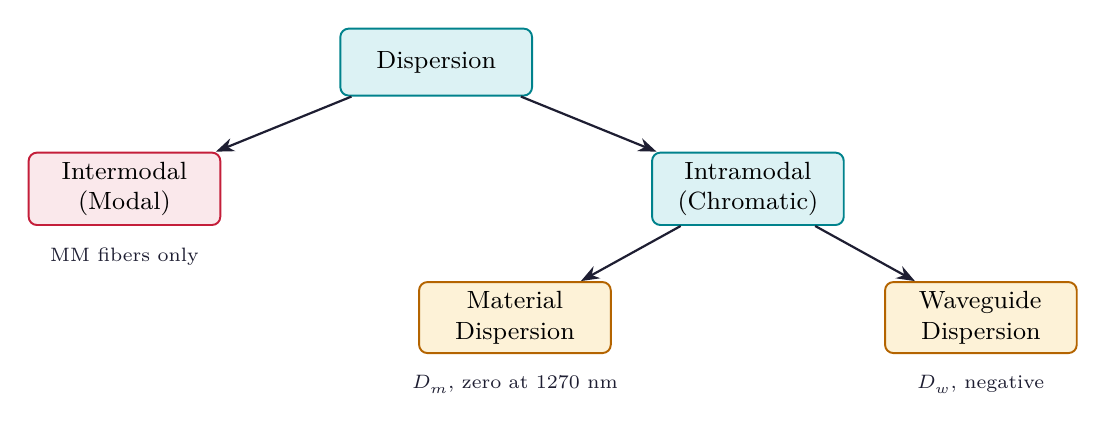
\begin{tikzpicture}[node distance=0.5cm and 0.7cm,
  sblock/.style={rectangle, draw=myteal, fill=hdrteal, text width=2.2cm,
    align=center, minimum height=0.85cm, font=\small, rounded corners=3pt, line width=0.7pt},
  rblock/.style={rectangle, draw=myred, fill=hdrred, text width=2.2cm,
    align=center, minimum height=0.85cm, font=\small, rounded corners=3pt, line width=0.7pt},
  ablock/.style={rectangle, draw=myamber, fill=hdramber, text width=2.2cm,
    align=center, minimum height=0.85cm, font=\small, rounded corners=3pt, line width=0.7pt}]
  \node[sblock] (disp) {Dispersion};
  \node[rblock, below left=0.7cm and 1.5cm of disp] (inter) {Intermodal\\(Modal)};
  \node[sblock, below right=0.7cm and 1.5cm of disp] (intra) {Intramodal\\(Chromatic)};
  \node[ablock, below left=0.7cm and 0.5cm of intra] (mat) {Material\\Dispersion};
  \node[ablock, below right=0.7cm and 0.5cm of intra] (wvg) {Waveguide\\Dispersion};
  \draw[arrow] (disp) -- (inter);
  \draw[arrow] (disp) -- (intra);
  \draw[arrow] (intra) -- (mat);
  \draw[arrow] (intra) -- (wvg);
  \node[font=\scriptsize\color{mydark}, below=0.15cm of inter] {MM fibers only};
  \node[font=\scriptsize\color{mydark}, below=0.15cm of mat] {$D_m$, zero at 1270 nm};
  \node[font=\scriptsize\color{mydark}, below=0.15cm of wvg] {$D_w$, negative};
\end{tikzpicture}
\end{tcolorbox}

% ===============================================================================
\section{Fiber Fabrication Processes}
% ===============================================================================

\begin{tcolorbox}[defbox, title={\textbf{Overview of Fabrication Methods}}]
Modern silica optical fibers are made by \textbf{Chemical Vapor Deposition (CVD)} processes, where dopant-laden gases react at high temperature to deposit glass layers. The four main processes are MCVD, OVD, VAD, and PCVD.
\end{tcolorbox}

\subsection{MCVD --- Modified Chemical Vapor Deposition}
Dopant gases (SiCl$_4$, GeCl$_4$, POCl$_3$, BCl$_3$) are flowed inside a silica tube. An external oxygen--hydrogen flame traverses the tube, causing oxidation and deposition of glass soot inside. Multiple passes deposit core and cladding layers. The tube is then collapsed into a solid \textbf{preform} by heating to $>2000^\circ$C.

\subsection{OVD --- Outside Vapor Deposition}
Soot is deposited on the \textbf{outside} of a bait rod (mandrel) via a flame hydrolysis burner. The rod is removed and the porous soot boule is consolidated (sintered) in a furnace to form a clear glass preform, then drawn into fiber.

\subsection{VAD --- Vapor Phase Axial Deposition}
Soot is deposited axially at the end of a rotating preform billet using burners. The porous preform grows \textbf{upward} and is continuously pulled into a consolidation furnace. Allows continuous fiber production. Produces very low OH$^-$ content.

\subsection{PCVD --- Plasma Chemical Vapor Deposition}
Uses a non-resonant microwave plasma (instead of a flame) inside a silica tube to drive the CVD reaction. Very precise compositional control; used for special fibers.

\par\noindent
{\renewcommand{\arraystretch}{1.55}
\begin{tabularx}{\linewidth}{|B{2.5cm}|Y|Y|Y|Y|}
\hline
\textbf{Feature} & \textbf{MCVD} & \textbf{OVD} & \textbf{VAD} & \textbf{PCVD} \\
\hline
Deposition location & Inside tube & Outside rod & Axial end & Inside tube \\
\hline
Heat source & External flame & Flame hydrolysis & Flame & Microwave plasma \\
\hline
Collapse needed? & Yes & Yes (soot) & Yes & Yes \\
\hline
OH$^-$ impurity & Moderate & Low & Very low & Low \\
\hline
Production rate & Medium & High & High (continuous) & Low \\
\hline
Profile control & Good & Good & Good & Excellent \\
\hline
\end{tabularx}}

% ===============================================================================
\section{Fiber Measurement Techniques}
% ===============================================================================

\begin{tcolorbox}[defbox, title={\textbf{Optical Time-Domain Reflectometer (OTDR)}}]
An OTDR is a sophisticated instrument that characterizes a fiber by injecting a short optical pulse and measuring the Rayleigh backscattered and Fresnel-reflected light as a function of time (and hence distance). It gives a \textbf{complete loss profile} of the fiber from a single end.
\end{tcolorbox}

\subsection{OTDR --- Principle and Trace Analysis}
The OTDR launches a pulse into the fiber. Light is continuously backscattered toward the OTDR. Splice losses, connector losses, and faults appear as steps or spikes. The time delay $t$ between launch and detection corresponds to a distance $d = ct/(2n_1)$.

\begin{tcolorbox}[tikzbox, title={Typical OTDR Trace}]
\centering
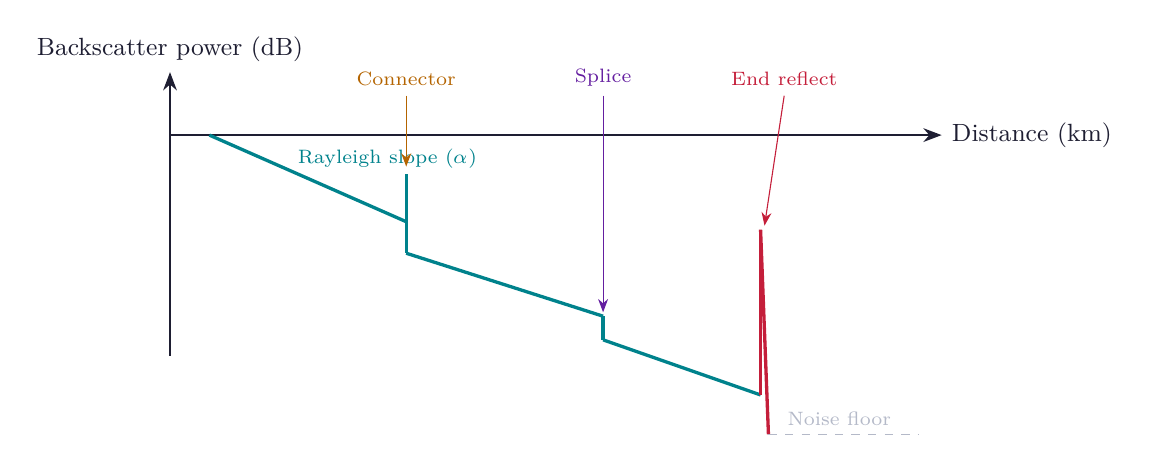
\begin{tikzpicture}[scale=1.0]
  % Axes
  \draw[-Stealth, thick, color=mydark] (0,0) -- (9.8,0) node[right,font=\small] {Distance (km)};
  \draw[-Stealth, thick, color=mydark] (0,-2.8) -- (0,0.8) node[above,font=\small] {Backscatter power (dB)};
  % Rayleigh backscatter slope
  \draw[very thick, color=myteal] (0.5,0.0) -- (3.0,-1.1);
  % Connector event (small spike up, then step down)
  \draw[very thick, color=myteal] (3.0,-1.1) -- (3.0,-0.5);
  \draw[very thick, color=myteal] (3.0,-0.5) -- (3.0,-1.5);
  \draw[very thick, color=myteal] (3.0,-1.5) -- (5.5,-2.3);
  % Splice event (step down, no spike)
  \draw[very thick, color=myteal] (5.5,-2.3) -- (5.5,-2.6);
  \draw[very thick, color=myteal] (5.5,-2.6) -- (7.5,-3.3);
  % End reflection (Fresnel peak then drop to noise floor)
  \draw[very thick, color=myred] (7.5,-3.3) -- (7.5,-1.2);
  \draw[very thick, color=myred] (7.5,-1.2) -- (7.6,-3.8);
  \draw[dashed, thin, color=mgframe] (7.6,-3.8) -- (9.5,-3.8);
  % Annotations
  \node[font=\scriptsize\color{myteal}, above right] at (1.5,-0.55) {Rayleigh slope ($\alpha$)};
  \draw[thin, -Stealth, color=myamber] (3.0, 0.5) -- (3.0, -0.4);
  \node[font=\scriptsize\color{myamber}, above] at (3.0, 0.5) {Connector};
  \draw[thin, -Stealth, color=mypurple] (5.5, 0.5) -- (5.5, -2.25);
  \node[font=\scriptsize\color{mypurple}, above] at (5.5, 0.5) {Splice};
  \draw[thin, -Stealth, color=myred] (7.8, 0.5) -- (7.55, -1.15);
  \node[font=\scriptsize\color{myred}, above] at (7.8, 0.5) {End reflect};
  \node[font=\scriptsize\color{mgframe}] at (8.5, -3.6) {Noise floor};
\end{tikzpicture}
\end{tcolorbox}

\textbf{Key OTDR terms:}
\begin{itemize}[leftmargin=*, itemsep=2pt]
  \item \textbf{Dead zone:} Distance near the launch connector where the receiver is saturated after a large Fresnel reflection --- events within this zone cannot be detected. Typical: 1--10\,m.
  \item \textbf{Dynamic range:} The difference between the initial backscatter power level and the noise floor (dB). Larger dynamic range $\Rightarrow$ longer fiber can be characterized.
\end{itemize}

\subsection{Cutback Method --- Attenuation Measurement}
The most accurate method for measuring attenuation. Launch power $P_1$ is measured by cutting the fiber close to the input ($\sim$2\,m from the source). Then the full-length measurement $P_2$ is taken. No need to disturb the launch conditions.
\[
\alpha = \frac{10}{L}\log_{10}\!\left(\frac{P_1}{P_2}\right) \quad\text{dB/km}
\]

\subsection{Interferometric Method --- Dispersion Measurement}
Used to measure \textbf{group delay} vs.\ wavelength. A broadband or tunable source illuminates the fiber; the output is compared against a reference path in a Mach-Zehnder or Michelson interferometer. Phase shift vs.\ wavelength gives the group delay $\tau(\lambda)$, from which $D(\lambda) = (1/L)\,d\tau/d\lambda$ (ps/nm$\cdot$km).

% ===============================================================================
% QUICK REVISION PAGE
% ===============================================================================
\newpage
\begin{center}
  {\large\bfseries\color{myred} Quick Revision --- Module 2}\\[3pt]
  {\small\color{mydark} Signal Degradation, Fabrication, and Measurement $|$ PE-EC801B}
\end{center}
\noindent{\color{myred}\rule{\linewidth}{1.2pt}}
\vspace{4pt}

\begin{tcolorbox}[formulabox, title={\textbf{Key Formulas at a Glance}}]
\renewcommand{\arraystretch}{1.35}
\begin{tabularx}{\linewidth}{B{5.0cm} X}
Attenuation coefficient & $\alpha = \displaystyle\frac{10}{L}\log_{10}(P_{in}/P_{out})$ \quad (dB/km) \\[6pt]
Output power & $P_{out} = P_{in} \cdot 10^{-\alpha L/10}$ \\[4pt]
Rayleigh scattering & Varies as $\lambda^{-4}$ \\[4pt]
RMS pulse spread & $\sigma = D \cdot L \cdot \Delta\lambda$ \\[4pt]
Modal dispersion (MMSI) & $\delta\tau = n_1 L \Delta / c$ \\[4pt]
Modal dispersion (MMGI) & $\delta\tau \approx n_1 L \Delta^2 / (2c)$ \\[4pt]
Chromatic dispersion & $D = D_m + D_w$ \quad (ps/nm$\cdot$km) \\[4pt]
BW--length product & $B \cdot L \leq 0.44/(\sigma/L)$ \\[4pt]
OTDR distance & $d = ct / (2n_1)$ \\[4pt]
\end{tabularx}
\end{tcolorbox}

\begin{tcolorbox}[defbox, title={\textbf{One-Line Definitions}}]
\begin{itemize}[leftmargin=*, itemsep=2pt, topsep=0pt]
  \item \textbf{Attenuation:} Reduction in optical power along the fiber; expressed in dB/km.
  \item \textbf{Rayleigh scattering:} Scattering from density fluctuations; $\propto \lambda^{-4}$; dominant at short $\lambda$.
  \item \textbf{Modal dispersion:} Pulse broadening from different modes arriving at different times; absent in SMF.
  \item \textbf{Material dispersion:} Pulse broadening due to $n(\lambda)$ variation; zero at 1270\,nm in silica.
  \item \textbf{Waveguide dispersion:} Pulse broadening due to wavelength-dependent propagation constant.
  \item \textbf{OTDR:} Instrument that measures fiber loss profile from a single end using backscattered light.
  \item \textbf{Dead zone:} Region near the OTDR launch where saturation prevents event detection.
  \item \textbf{Cutback method:} Gold-standard destructive technique for measuring fiber attenuation accurately.
  \item \textbf{MCVD:} Modified CVD --- glass deposited inside a silica tube by an external traversing flame.
\end{itemize}
\end{tcolorbox}

\begin{tcolorbox}[exambox, title={\textbf{Frequently Asked / Viva Questions}}]
\begin{enumerate}[topsep=0pt, label=\textbf{Q\arabic*.}, itemsep=5pt]
  \item \Q{What are the main causes of attenuation in an optical fiber?}
    Absorption (intrinsic UV/IR resonances and extrinsic OH$^-$ impurities), Rayleigh scattering ($\lambda^{-4}$), Mie scattering, macrobending, and microbending losses.
  \item \Q{Why is 1310\,nm and 1550\,nm preferred as operating windows?}
    At 1310\,nm, chromatic dispersion is near zero for SMF. At 1550\,nm, Rayleigh scattering is low, giving minimum attenuation ($\sim$0.2\,dB/km) for standard silica SMF.
  \item \Q{What is Rayleigh scattering and why is it important?}
    It results from random sub-wavelength density fluctuations in silica. Since it varies as $\lambda^{-4}$, it is the dominant loss at short wavelengths and sets the lower limit for SMF attenuation.
  \item \Q{Distinguish between intermodal and intramodal dispersion.}
    Intermodal dispersion occurs in multimode fibers when different modes travel at different velocities. Intramodal (chromatic) dispersion occurs within a single mode due to material and waveguide effects.
  \item \Q{Why does MMGI have lower modal dispersion than MMSI?}
    The parabolic index profile of MMGI makes higher-order modes travel faster (in lower-index outer regions), nearly equaling the speed of lower-order modes. This self-focusing effect reduces differential mode delay.
  \item \Q{What is bandwidth--length product? Give a typical value.}
    It is the product $B \times L$ (MHz$\cdot$km or GHz$\cdot$km), measuring the information capacity of a fiber per unit length. Typical: MMSI $\sim$20\,MHz$\cdot$km; MMGI $\sim$1000\,MHz$\cdot$km; SMF $>$100\,GHz$\cdot$km.
  \item \Q{Explain the OTDR principle briefly.}
    A short optical pulse is launched into the fiber. The OTDR measures the time-resolved backscattered signal. Distance is calculated as $d = ct/(2n)$. The trace shows attenuation slope, splices, connectors, and fiber end.
  \item \Q{What is the dead zone in an OTDR?}
    The dead zone is the distance near the OTDR launch connector where the receiver is saturated by the large Fresnel reflection, making it unable to detect nearby events. Typically 1--10\,m.
  \item \Q{Describe the cutback method for attenuation measurement.}
    Launch power $P_1$ is measured by cutting the fiber $\sim$2\,m from the source. Then full-length output $P_2$ is measured. $\alpha = (10/L)\log(P_1/P_2)$. Most accurate but destructive.
  \item \Q{What is the difference between macrobending and microbending?}
    Macrobending is a large-radius bend that causes the evanescent field to radiate. Microbending consists of random small-amplitude axis deformations from cabling stress, causing mode coupling and loss.
  \item \Q{What is MCVD? How is the preform made?}
    Modified CVD. Dopant gases flow inside a rotating silica tube; an external oxy-hydrogen flame deposits glass soot on the inner wall. Multiple passes build up core/cladding layers, then the tube is collapsed into a solid preform.
\end{enumerate}
\end{tcolorbox}

\begin{tcolorbox}[tikzbox, title={Comparison: Fabrication Methods}]
\centering
{\renewcommand{\arraystretch}{1.45}
\begin{tabularx}{\linewidth}{|B{2.2cm}|Y|Y|Y|Y|}
\hline
\textbf{Method} & \textbf{Deposition} & \textbf{Heat Source} & \textbf{OH$^-$} & \textbf{Rate} \\
\hline
MCVD & Inside tube & External flame & Moderate & Medium \\
\hline
OVD & Outside rod & Flame hydrolysis & Low & High \\
\hline
VAD & Axial end & Flame & Very low & High (cont.) \\
\hline
PCVD & Inside tube & Microwave plasma & Low & Low \\
\hline
\end{tabularx}}
\end{tcolorbox}

\end{document}
